\documentclass[svgnames,11pt]{beamer}
\input{/home/tof/Documents/Cozy/latex-include/preambule_commun.tex}
\input{/home/tof/Documents/Cozy/latex-include/preambule_beamer.tex}
%\usepackage{pgfpages} \setbeameroption{show notes on second screen=left}
\author[]{Christophe Viroulaud}
\title{Exponentiation \\Notion de récursivité}
\date{\framebox{\textbf{Lang 05}}}
%\logo{}
\institute{Terminale - NSI}

\begin{document}
\begin{frame}
\titlepage
\end{frame}
\begin{frame}
    \frametitle{}
L'\emph{exponentiation} est une opération mathématique définie par:
    $$a^n=\underbrace{a ×....× a}_{\mbox{n fois}}\qquad et\ a^0=1$$

\note{Un calcul comme $3^4$ ne pose pas de problème mais $2701^{103056}$ peut prendre un certain à effectuer par le langage de programmation.}

\end{frame}
\begin{frame}
    \frametitle{}

    \begin{itemize}
        \item $2^4 \rightarrow$ 3 opérations,
        \item $2701^{103056} \rightarrow$ 103055 opérations.
    \end{itemize}
\begin{framed}\centering Comment calculer la puissance d'un nombre de manière optimisée?
\end{framed}
\end{frame}
\section{Étude de la fonction native}
\subsection{Fonctions  Python "built-in"}
\begin{frame}[fragile]
    \frametitle{Fonctions  Python "built-in"}

\begin{center}
\begin{lstlisting}[language=Python , basicstyle=\ttfamily\small, xleftmargin=2em, xrightmargin=2em]
def puissance_star(x:int,n:int)->int:
    return x**n

def puissance_builtin(x:int,n:int)->int:
    return pow(x,n)
\end{lstlisting}
\captionof{code}{Fonctions natives}
\label{builtin}
\end{center}
\begin{activite}
Tester les deux fonctions du code \ref{builtin}.
\end{activite}
\end{frame}
\subsection{Tester un programme}
\subsubsection{Préconditions}
\begin{frame}
    \frametitle{Préconditions}

    Nous décidons de nous limiter au cas positif.
    \begin{aretenir}[]
        La programmation \emph{défensive} consiste à anticiper les problèmes éventuels.
    \end{aretenir}
    \begin{activite}
        Mettre en place un test qui lèvera une \textbf{\texttt{AssertionError}} si l'exposant est négatif.
        \end{activite}
        
\end{frame}
\begin{frame}[fragile]
    \frametitle{Correction}

\begin{center}
\begin{lstlisting}[language=Python , basicstyle=\ttfamily\small, xleftmargin=1em, xrightmargin=0.5em]
def puissance_star(x: int, n: int) -> int:
    assert n >= 0, "L'exposant doit être positif."
    return x**n
\end{lstlisting}
\captionof{code}{}
\label{CODE}
\end{center}

\end{frame}
\subsubsection{Mettre en place des tests}
\begin{frame}
    \frametitle{Mettre en place des tests}

    Il existe plusieurs modules (\textbf{\texttt{doctest}}) qui facilitent les phases de test.   

\end{frame}
\begin{frame}[fragile]
    \frametitle{}

    \begin{center}
    \begin{lstlisting}[language=Python , basicstyle=\ttfamily\small, xleftmargin=2em, xrightmargin=2em]
import doctest

def puissance_star(x:int,n:int)->int:
    """
    >>> puissance_star(2,8)
    256
    >>> puissance_star(2,9)
    512
    """
    return x**n

doctest.testmod(verbose=True)
\end{lstlisting}
    \captionof{code}{Tester une fonction}
    \label{CODE}
    \end{center}

\end{frame}
\subsubsection{Durée d'exécution}
\begin{frame}
    \frametitle{Durée d'exécution}

\begin{activite}
À l'aide de la bibliothèque \textbf{\texttt{time}} mesurer la durée d'exécution de la fonction \textbf{\texttt{puissance\_star}} pour calculer $2701^19406$.
\end{activite}

\end{frame}
\begin{frame}[fragile]
    \frametitle{Correction}

\begin{center}
\begin{lstlisting}[language=Python , basicstyle=\ttfamily\small, xleftmargin=2em, xrightmargin=2em]
from time import time

debut=time()
puissance_star(2701,19406)
fin=time()
print("opérande **",fin-debut)
\end{lstlisting}
\label{CODE}
\end{center}

\end{frame}
\section{Implémenter la fonction \emph{puissance}}
\subsection{S'appuyer sur la définition mathématique}
\begin{frame}
    \frametitle{S'appuyer sur la définition mathématique}

    $$a^n=\underbrace{a ×....× a}_{n fois}\qquad et \qquad a^0=1$$
    \begin{activite}
    \begin{enumerate}
    \item Implémenter la fonction \textbf{puissance\_perso(x: int, n: int)\;\rightarrow\;int} sans utiliser les fonctions buitin de Python.
    \item Mettre en place un test de vérification de la fonction.
    \item Mesurer le temps d'exécution de la fonction en l'appelant avec les paramètres (2701,19406).
    \end{enumerate}
    \end{activite}

\end{frame}
\begin{frame}[fragile]
    \frametitle{Correction}

\begin{center}
\begin{lstlisting}[language=Python , basicstyle=\ttfamily\small, xleftmargin=2em, xrightmargin=2em]
def puissance_perso(x:int,n:int)->int:
    """
    >>> puissance_perso(2,8)
    256
    >>> puissance_perso(2,9)
    512
    """
    res = 1
    for i in range(n):
        res*=x
    return res
\end{lstlisting}
\end{center}
\begin{center}
\begin{lstlisting}[language=Python , basicstyle=\ttfamily\small, xleftmargin=2em, xrightmargin=2em]
opérande ** 0.006058692932128906
fonction pow() 0.005688667297363281
fonction personnelle 0.13074541091918945
\end{lstlisting}
\captionof{code}{Les résultats sont significatifs.}
\label{CODE}
\end{center}
\end{frame}
\subsection{Correction de l'algorithme}
\begin{frame}
    \frametitle{Correction de l'algorithme}

    \begin{aretenir}[]
        Un \textbf{invariant de boucle} est une propriété qui si elle est vraie avant l’exécution d’une itération le demeure après l’exécution de l’itération.
    \end{aretenir}

\end{frame}
\begin{frame}[fragile]
    \frametitle{}

    \begin{center}
    \begin{lstlisting}[language=Python , basicstyle=\ttfamily\small, xleftmargin=2em, xrightmargin=2em]
res = 1
for i in range(n):
    res*=x
\end{lstlisting}
    \captionof{code}{La propriété $res = x^i$ est un invariant de boucle.}
    \label{CODE}
    \end{center}
\note{C'est en fait un raisonnement par récurrence comme en mathématiques.}
\end{frame}
\section{Formulations récursives}
\subsection{Notation mathématique}
\begin{frame}
    \frametitle{Notation mathématique}

    $$
    puissance(x,n) = \left\{
        \begin{array}{ll}
            1 & \mbox{si } n=0 \\
            x.puissance(x,n-1) & \mbox{si } n>0
        \end{array}
    \right.
    $$
\begin{aretenir}[]
Une fonction \textbf{récursive} est une fonction qui s'appelle elle-même.
\end{aretenir}   
\note{récursivité = technique de programmation // impératif}
\end{frame}
\subsection{Implémentation}
\begin{frame}
    \frametitle{Implémentation}

\begin{aretenir}[]
Une fonction récursive:
\begin{itemize}
    \item s'appelle elle-même,
    \item possède un \textbf{cas limite} pour stopper les appels.
\end{itemize}
\end{aretenir}

\end{frame}
\begin{frame}[fragile]
    \frametitle{}

    \begin{center}
    \begin{lstlisting}[language=Python , basicstyle=\ttfamily\small, xleftmargin=2em, xrightmargin=1em]
def puissance_recursif(x: int, n: int) -> int:
    if n == 0: # cas limite
        return 1
    else: # appel récursif
        return x*puissance_recursif(x, n-1)
\end{lstlisting}
    \captionof{code}{Traduction de la formule mathématique}
    \label{CODE}
    \end{center}

\end{frame}
\begin{frame}[fragile]
    \frametitle{Pile d'appels}

\begin{center}
\centering
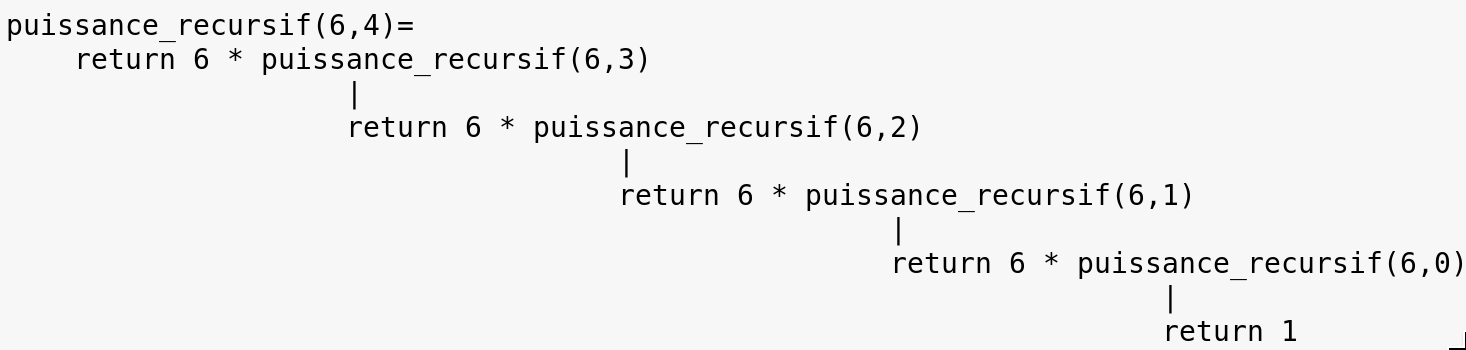
\includegraphics[width=10cm]{ressources/pile-appels.png}

\end{center}
\begin{center}
    \href{http://pythontutor.com/visualize.html#code=def%20puissance_recursif%28x%3A%20int,%20n%3A%20int%29%20-%3E%20int%3A%0A%20%20%20%20if%20n%20%3D%3D%200%3A%20%23%20cas%20limite%0A%20%20%20%20%20%20%20%20return%201%0A%20%20%20%20else%3A%20%23%20appel%20r%C3%A9cursif%0A%20%20%20%20%20%20%20%20return%20x*puissance_recursif%28x,%20n-1%29%0A%0Apuissance_recursif%286,4%29&cumulative=false&curInstr=0&heapPrimitives=nevernest&mode=display&origin=opt-frontend.js&py=3&rawInputLstJSON=%5B%5D&textReferences=false}{Visualisation}
\end{center}

\end{frame}
\begin{frame}
    \frametitle{}

    \begin{aretenir}[]
        La \textbf{pile d'appels} stocke les appels successifs de la fonction récursive.
        \end{aretenir}

\end{frame}
\begin{frame}[fragile]
    \frametitle{}

    \begin{aretenir}[Remarques]
    \begin{itemize}
        \item<1-> Python limite la pile d'appels à 1000 récursions.
\begin{center}
\begin{lstlisting}[language=Python , basicstyle=\ttfamily\small, xleftmargin=2em, xrightmargin=2em]
import sys
sys.setrecursionlimit(20000)
\end{lstlisting}
\captionof{code}{Augmenter le nombre de récursions}
\label{CODE}
\end{center}
        \item<2-> La durée d'exécution ne s'est pas améliorée.
\begin{center}
\begin{lstlisting}[language=Python , basicstyle=\ttfamily\small, xleftmargin=2em, xrightmargin=2em]
fonction récursive 0.16802310943603516
\end{lstlisting}
\end{center}
    \end{itemize}
    \end{aretenir}
\note[item]{Il n'y a pas de raison que ça soit mieux: le nombre d'opérations reste le même}
\note[item]{même un peu moins bien: la récursivité est moins bien géré par l'interpréteur Python que par d'autres langages (Ocaml)}
\end{frame}
\subsection{Nouvelle formulation mathématique}
\begin{frame}
    \frametitle{Nouvelle formulation mathématique}

    \begin{figure}[!h]
        \centering
        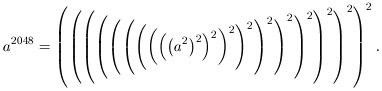
\includegraphics[width=10cm]{ressources/exponentiationrapide.png}
        \captionof{figure}{Exponentiation rapide}
        \label{exponentiation}
        \end{figure}

\end{frame}
\begin{frame}
    \frametitle{}

    $$
puissance(x,n) = 
$$
$$\left\{
    \begin{array}{ll}
        1 & \mbox{si } n=0 \\
        puissance(x*x,n/2) & \mbox{si } n>0 \mbox{ et n pair}\\
        x.puissance(x*x,(n-1)/2) & \mbox{si } n>0 \mbox{ et n impair}\
    \end{array}
\right.$$
\begin{activite}
Implémenter la fonction \textbf{\texttt{puissance\_recursif\_rapide(x: int, n: int)$\rightarrow$ int }} qui traduit la formulation récursive précédente.
\end{activite}

\end{frame}
\begin{frame}[fragile]
    \frametitle{Correction}

\begin{center}
\begin{lstlisting}[language=Python , basicstyle=\ttfamily\small, xleftmargin=0.5em, xrightmargin=0.5em]
def puissance_recursif_rapide(x: int, n: int) -> int:
    if n == 0: # cas limite
        return 1
    elif n % 2 == 0: # pair
        return puissance_recursif_rapide(x*x, n//2)
    else: # impair
        return x*puissance_recursif_rapide(x*x, n//2)
\end{lstlisting}
\captionof{code}{Exponentiation rapide}
\label{CODE}
\end{center}
\begin{center}
    \href{https://pythontutor.com/visualize.html#code=def%20puissance_recursif_rapide%28x,%20n%29%3A%0A%20%20%20%20if%20n%20%3D%3D%200%3A%0A%20%20%20%20%20%20%20%20return%201%0A%20%20%20%20elif%20n%20%25%202%20%3D%3D%200%3A%0A%20%20%20%20%20%20%20%20return%20puissance_recursif_rapide%28x*x,%20n//2%29%0A%20%20%20%20else%3A%0A%20%20%20%20%20%20%20%20return%20x*puissance_recursif_rapide%28x*x,%20n//2%29%0A%0Apuissance_recursif_rapide%283,%205%29&cumulative=false&curInstr=0&heapPrimitives=nevernest&mode=display&origin=opt-frontend.js&py=3&rawInputLstJSON=%5B%5D&textReferences=false}{Visualisation}
\end{center}
\end{frame}
\begin{frame}[fragile]
    \frametitle{}

    \begin{center}
        \begin{lstlisting}[language=Python , basicstyle=\ttfamily\small, xleftmargin=2em, xrightmargin=2em]
fonction récursive rapide 0.021007537841796875
\end{lstlisting}
        \captionof{code}{Les résultats s'améliorent sans égaler la fonction native.}
        \label{CODE}
        \end{center}
\note[item]{Implémentation des fonctions builtin en C}
\note[item]'itératif plus rapide car appels fonction coûtent; mais récursif donne souvent code plus clair/lisible
\end{frame}
\end{document}